\section{Modelo AS-IS}

\subsection{Modelos dos processos}
Nessa seção vamos abordar a modelagem dos processos identificados no contexto,
os processos aqui mostrados usam a notação do BPMN para dar clareza e objetividade.
Proporcionando um padrão internacional de leitura dos mesmos.

\subsubsection{Gerência de requisição}
\begin{figure}[!h]
\caption{Gerencia de requisição}
\centering % para centralizarmos a figura
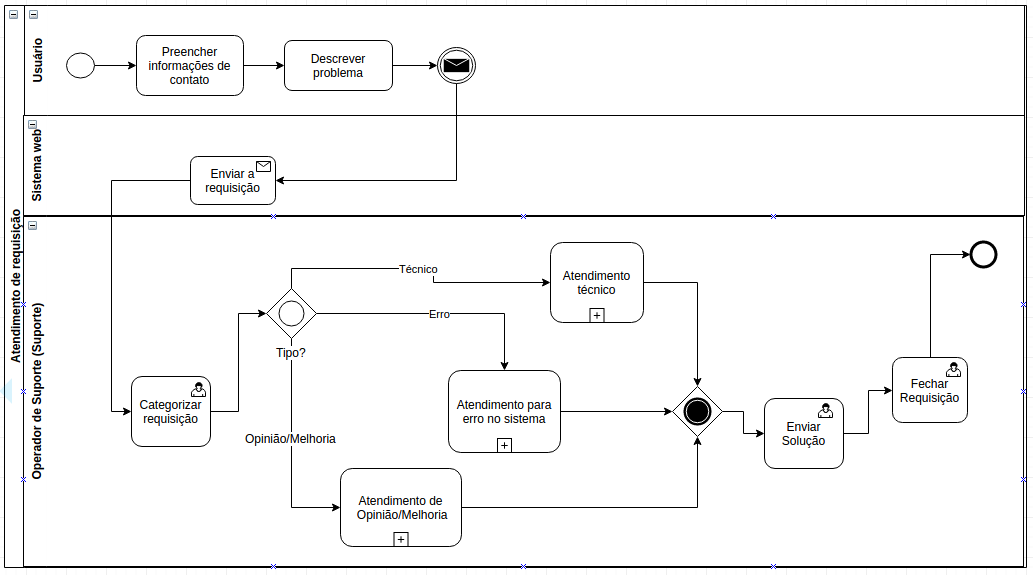
\includegraphics[width=15cm]{as-is/01_atendimento_de_requisicao.png}
\label{figura:atendimento_requisicao_as_is}
\end{figure}

\begin{itemize}[noitemsep]
	\item Preencher informações de contato
		\begin{itemize}
			\item O usuário preenche um formulário com o nome, email e telefone de contato
		\end{itemize}
	\item Descrever problema
		\begin{itemize}
			\item Realiza a descrição do problema
		\end{itemize}
	\item Enviar requisição
		\begin{itemize}
			\item O sistema web envia um email para o operador
		\end{itemize}
	\item Categorizar requisição
		\begin{itemize}
			\item Atribui uma categoria correta a requisição
		\end{itemize}
	\item Enviar Solicitação
		\begin{itemize}
			\item Envia informação sobre a decisão/solução
		\end{itemize}
	\item Fechar requisição
		\begin{itemize}
			\item Marca como finalizada a requisição
		\end{itemize}
\end{itemize}


\subsubsection{Atendimento técnico}

\begin{figure}[!h]
\caption{Atendimento técnico}
\centering % para centralizarmos a figura
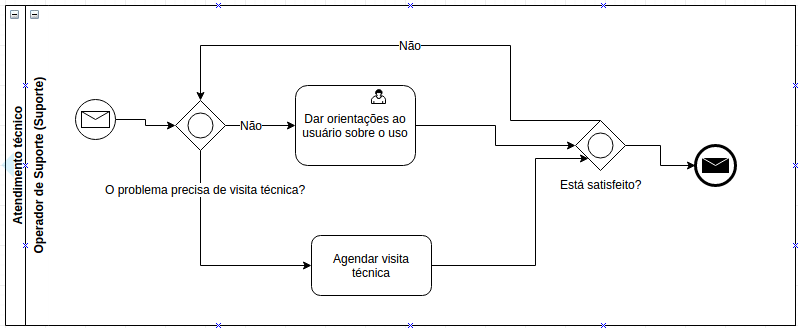
\includegraphics[width=15cm]{as-is/02_atendimento_tecnico.png}
\label{figura:suporte_tecnico_as_is}
\end{figure}

\begin{itemize}[noitemsep]
	\item Dar orientações ao usuário sobre o uso
		\begin{itemize}
			\item Dar orientações para que o usuário possa resolver um problema de uso
		\end{itemize}
	\item Agendar visita técnica
		\begin{itemize}
			\item Marcar data para a realização de uma visita
		\end{itemize}
\end{itemize}

\subsubsection{Atendimento para erro no sistema}
\begin{figure}[!h]
\caption{Atendimento para erro no sistema}
\centering % para centralizarmos a figura
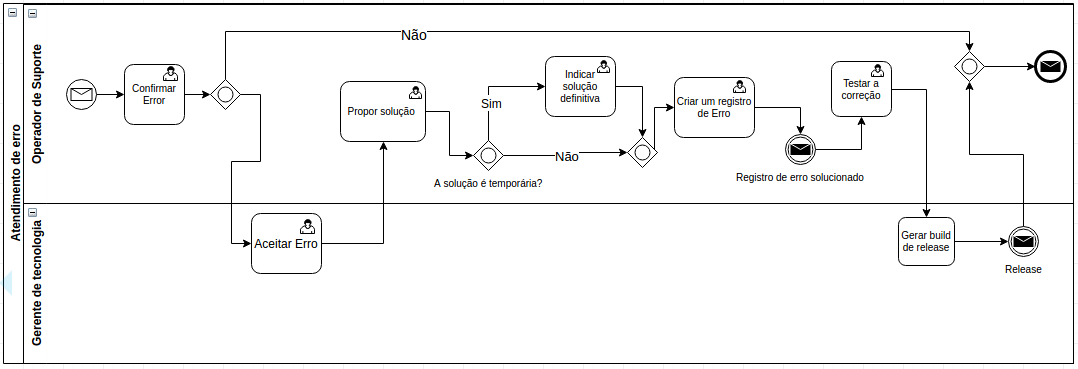
\includegraphics[width=16cm, height=5cm]{as-is/03_atendimento_de_erro.png}
\label{figura:atendimento_de_erro_as_is}
\end{figure}

\begin{itemize}[noitemsep]
	\item Confirmar erro
		\begin{itemize}
			\item Confirma se o erro realmente existe
		\end{itemize}
	\item Aceitar Erro
		\begin{itemize}
			\item Aceita a existência do erro e planeja a correção
		\end{itemize}
	\item Propor Solução
		\begin{itemize}
			\item E discutida uma solução, para ser implantada rapidamente
		\end{itemize}
	\item Indicar Solução definitiva
		\begin{itemize}
			\item Indica a melhor solução para o problema
		\end{itemize}
	\item Criar registro
		\begin{itemize}
			\item E registrado o erro solucionado
		\end{itemize}
	\item Testar correção
		\begin{itemize}
			\item E realizado testes que comprovem a correção do erro
		\end{itemize}
	\item Gerar build de release
		\begin{itemize}
			\item E disponibilizado para os clientes a versão atualizada
		\end{itemize}
\end{itemize}
\clearpage
\subsubsection{Atendimento de Opinião/Melhoria}

\begin{figure}[!h]
\caption{Atendimento de Opinião/Melhoria}
\centering % para centralizarmos a figura
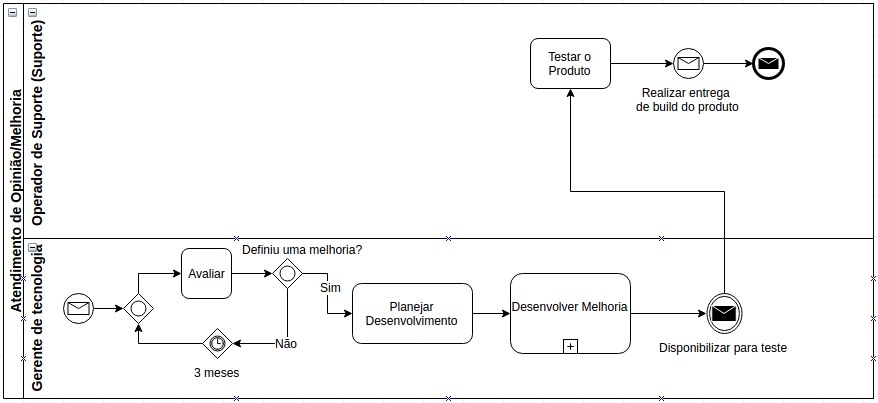
\includegraphics[width=15cm]{as-is/04_atendimento_de_melhoria.png}
\label{figura:atendimento_de_melhoria_as_is}
\end{figure}

\begin{itemize}[noitemsep]
	\item Avaliar
		\begin{itemize}
			\item Avaliar a proposta
		\end{itemize}
	\item Planejar Desenvolvimento
		\begin{itemize}
			\item E planejado o desenvolvimento da melhoria
		\end{itemize}
	\item Testar o produto
			\begin{itemize}
				\item E realizado testes que comprovem a adição da melhoria
			\end{itemize}
\end{itemize}


\subsection{Conclusão e análise - AS-IS}
\begin{itemize}[noitemsep]
  \item Processos indefinidos
  \item Ausência de monitoramentos
  \item Ausência de autenticação de usuário
  \item Processos de longo tempo de execução
  \item Reporte insuficiênte para o cliente
\end{itemize}
